\documentclass[a4paper,11pt]{article}

\input ../include/preamble.tex

\usepackage{tikz}
\usetikzlibrary{automata,arrows,topaths,calc,positioning}

\usepackage{circuitikz}

\usepackage{subcaption}

\usepackage{changepage}

\usepackage{listings}

\lstdefinelanguage{elixir}{
	morekeywords={case,catch,def,do,else,false,%
		use,alias,receive,timeout,defmacro,defp,%
		for,if,import,defmodule,defprotocol,%
		nil,defmacrop,defoverridable,defimpl,%
		super,fn,raise,true,try,end,with,%
		unless},
	otherkeywords={<-,->},
	sensitive=true,
	morecomment=[l]{\#},
	morecomment=[n]{/*}{*/},
	morestring=[b]",
	morestring=[b]',
	morestring=[b]"""
}

\lstset{language=elixir}

\begin{document}

\title{
    \textbf{A MIPS emulator}\\
    \large{Programming II}
}
\author{Johan Montelius}
\date{Spring Term 2021}
\maketitle
\defaultpagestyle

\section{Introduction}

In this exercise we will combine your knowledge of computer
architecture and concurrent programming to implement an emulator of a
simple MIPS processor. You should have basic understanding of the
architecture and how the data path is implemented. We will only
implement a small subset of the MIPS machine instructions but it will
be possible to extend it.

\section{MIPS architecture}

There are of course many different ways a MIPS CPU can be designed but
we will follow the description given in chapter four of ``Computer
Organization and Design'' by Patterson and Hennessy. If you have not
studied their description you should do so before starting with the
implementation, this is not a tutorial of the MIPS architecture.


\subsection{high-level design}

We will divide the processor into five units, each unit will be
implemented as an Elixir process and the data-paths will be Elixir
messages. This might not be a straight forward way to implement an
emulator but it more challenging and you will learn a lot about
concurrency in Elixir.

The units, which will also be Elixir modules, are:

\begin{itemize}

\item {\bf Instruction} : instruction fetcher, will retrieve the next
  instruction, divide it into its parts and send them to other units.

\item {\bf Register} : reads the contents of the registers
  and passes the values to the ALU.

\item {\bf ALU} : performs the arithmetic operations and passes the
  result to the memory unit.

\item {\bf Memory} : handles load and store operation and in the case
  of a load, passes the read value to the register unit.

\item {\bf Branch} : decides which instruction to execute next. In the
  beginning this is simply the next instruction ({\em program counter
    + 4}) but when we introduce branch and jump instructions this unit
  will have more things to do.

\item {\bf Controller} : the brain of the CPU, will receive the op
  codes from the instruction unit and direct the other units what to do.
  
\end{itemize}

In Fig.\ref{fig:flow} we see an overview of the CPU with the primary
data flow. To simplify the image the messages from the control unit
to the other units are not drawn.

The execution will always start by a message from the branch unit to
the instruction unit. The message contains the value of the program
counter from which address the next instruction should be fetched.

The instruction unit will fetch the next instruction and send the
register identifiers to the register unit. It will also send a
possible immediate value directly to the ALU and the branch
unit. These immediate values might be used depending on the
instruction but it is not up to the instruction unit to decide.

The register unit will send the content of the registers to the ALU
unit but also pass one value directly to the memory unit. This will
typically be a value that should be stored. The ALU does its
computation and sends the result, and address, to the memory unit. It
will also send a message to the branch unit describing the outcome of
the operation i.e. if it was zero or not.

The memory unit will either store a value in memory or load a value
from memory. If it is a load instruction that is executed, it will
send the retrieved value back to the register unit. The register unit
will then store it in one of the registers.

The branch unit will receive both an immediate value from the
instruction unit and a value from the register unit. Depending on the
instruction, and the outcome of the ALU operation, the program counter
is updated.


\begin{figure}
  \centering 
  \begin{tikzpicture}[unit/.style={rectangle, very thick, minimum height=1cm, minimum width=2cm, text centered}]

%Nodes
\node[unit]    (instr)                      {Instruction};
\node[unit]    (reg)       [right=of instr] {Register};
\node[unit]    (alu)       [right=of reg]   {ALU};
\node[unit]    (mem)       [right=of alu]   {Memory};
\node[unit]    (brn)       [above=of alu]   {Branch};
\node[unit]    (ctrl)       [below=of reg]   {Controller};
%Lines 
\draw[->, dash dot] (instr.east) -- (reg.west);
\draw[->, dashed] (instr.south) .. controls +(down:1cm) and +(left:1cm) ..  (ctrl.west);

\draw[->] (reg.east) -- (alu.west);

\draw[->] (alu.east) -- (mem.west);
\draw[->, dashed] (alu.north) -- (brn.south);

\draw[->] (instr.north) .. controls +(up:1cm) and +(left:1cm) .. (brn.west);
\draw[->] (instr.south) .. controls +(down:1cm) and +(down:1cm) .. (alu.south);

\draw[->] (reg.south) .. controls +(down:1cm) and +(down:1cm) .. (mem.south);

\draw[->, dash dot] (brn.north) .. controls +(up:2cm) and +(left:3cm) .. (instr.west);
\draw[->] (mem.north) .. controls +(up:1cm) and +(up:1cm) .. (reg.north);

  \end{tikzpicture}
  \caption{The data flow of the processor.} \label{fig:flow}
\end{figure}

What each unit should do is of course determined by the controller
unit that is given the op code from the instruction unit. The controller is
normally described as two units, one main controller and a separate
ALU controller. We will combine these into one unit; nothing is gained
by separating them.

In addition to the units described we will have one {\em output
  unit}. In order to write small programs that actually returns a
result more than an updated memory, the ALU can be directed to send
values to the output. The output unit can either echo these values to
the terminal and/or save them and return them as a result of the
computation.

\subsection{signals as messages}

When you see the regular description of the CPU architecture you will
see how for example the instruction unit sends three different signals to
the register unit: source register, target register and destination register. We will
implement this in one message. The register unit will in the same way
pass two values to the ALU i one message.  Our implementation is thus
more focused on which information that is passed between the units
rather than how this would realized in a hardware implementation.


\subsection{the program}

In this implementation we will make things a bit easier by separating
the code from the main memory. In real life, the code is of course in
the main memory but it makes things easier if we keep them in two
different data structures. The only limitations that this will mean is
that 1/ we will not be able to change the code during execution and 2/
we can not use the program counter as a base address when accessing
data.

The first limitation is something we can live with, few programs write
to the code segment anyway. The second limitation could be a problem but
not in the MIPS architecture; there are no instructions that operate
relative to the program counter.

Since we will not write to the code area we can implement this with a
data structure that maximize read performance. The main memory
however, should be some data structure with efficient random read and
write operations. All things related to how instructions and data are
stored in memory will be in a module called {\tt Program}. This
module will also implement a {\em loader} that takes an assembler
description of a program and returns the {\em code} and {\em data}
structures.


\subsection{the controller}

The Controller is of course the heart of the system. It will receive
a message from the instruction unit with the op code and ALU function
code. It then determines what the different units should do and sends
the corresponding signals. This is how the units can be directed:

\begin{itemize}

\item {\bf Register} : the register unit can proceed and send the two
  values to the ALU but must then know if it should store the value
  returned from the memory unit and which register to store it in.

\item {\bf ALU} : the ALU must of course know which operation to
  perform but it must also know it it should use both values from the
  register unit or if it should use the immediate value from the
  instruction unit.

\item {\bf Memory} : the memory unit must know if it should perform a
  load, store or no-op. If it is a load instruction the read value
  should be returned to the register unit. If it is a store operation
  it does not matter what it outputs (but it must send a value)
  otherwise it sends the value it received from the ALU.

\item {\bf Branch} : the branch unit needs to know if the operation is a
  branch or jump instruction in order to determine how to select the
  next program counter; increment by four or jump.
  
\end{itemize}

\subsection{asynchronous pipeline}

One thing that we have not mentioned is how to time things, where is
the clock pulse and when should units proceed. The answer is that the
design is asynchronous and a unit can proceed as soon as it has the
available information.

Asynchronous does not mean chaos so we need to think about how this
should work. One example where things could go wrong is if the branch
unit decides to send the next program counter to the Instruction unit
since it knows it's not a branch instruction being executed - why wait
for the ALU if the zero information is not needed? The problem is if
the next instruction is a branch instruction and the zero message from
the previous instructions is read; we need a way to keep things
synchronized even though messages are sent asynchronous. 

To make this work we first of all rely on the ordered delivery of
messages. What ever happen, messages will not be delivered out of
order. Elixir does of course not guarantee that messages do arrive but
this is something that we will ignore, we work under the assumption
that all messages do arrive (which they will if we do not distribute
the system over a network).

To visualize the communication protocol we draw a sequence diagram. In
Fig.~\ref{fig:seq} we see all of the messages that are sent during one
instruction cycle. All of these messages should be sent and a unit
needs to receive them all. Note that the diagram only shows the
logical time relations. The register unit can not send the values $vs$
and $vt$ before receiving the register numbers from the Instruction
unit. However, nothing prevents the immediate value from the
Instruction unit to reach the ALU unit before the $va$ and $vt$
values. Moreover, all though in the diagram we have the register unit
first send the values to the ALU before sending the value to the
memory unit but this order is not important. Messages can take
arbitrary long time and as long as we're not sending two messages to
the same receiver, the order is irrelevant. 

\begin{figure}
  \centering 
  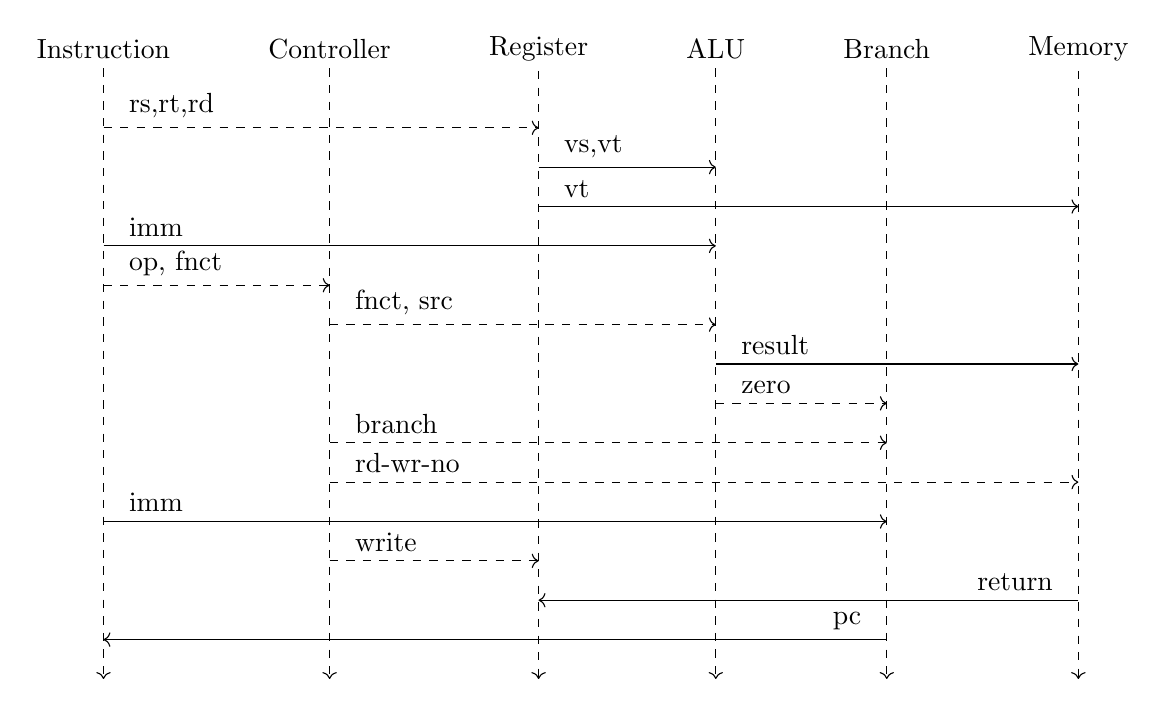
\begin{tikzpicture}[frw/.style={xshift=0.2cm, yshift=-0.1, anchor= south west}, bkw/.style={xshift=-0.2cm, anchor= south east}]

    \node[]                 (instr) {Instruction};
    \node[right = of instr] (ctrl)  {Controller};
    \node[right = of ctrl]  (reg)   {Register};
    \node[right = of reg]   (alu)   {ALU};    
    \node[right = of alu]   (brn)   {Branch};
    \node[right = of brn]   (mem)   {Memory};    
    
    
    \draw[->, dashed] (instr) -- ($ (instr) - (0,8)$);
    \draw[->, dashed] (reg) -- ($ (reg) - (0,8)$);
    \draw[->, dashed] (ctrl) -- ($ (ctrl) - (0,8)$);
    \draw[->, dashed] (alu) -- ($ (alu) - (0,8)$);
    \draw[->, dashed] (brn) -- ($ (brn) - (0,8)$);    
    \draw[->, dashed] (mem) -- ($ (mem) - (0,8)$);    
    
    \draw[->, dashed] ($(instr) - (0,1)$) node[frw]{rs,rt,rd} --  ($(reg)  - (0,1)$);

    \draw[->] ($(reg) - (0,1.5)$) node[frw]{vs,vt} --  ($(alu)  - (0,1.5)$);

    \draw[->] ($(reg) - (0,2.0)$) node[frw]{vt} --  ($(mem)  - (0,2.0)$);
    

    \draw[->] ($(instr) - (0,2.5)$) node[frw]{imm} --  ($(alu)  - (0,2.5)$);

    \draw[->, dashed] ($(instr) - (0,3.0)$) node[frw]{op, fnct}  --   ($(ctrl)  - (0,3.0)$);

    \draw[->, dashed] ($(ctrl) - (0,3.5)$) node[frw]{fnct, src} --  ($(alu)  - (0,3.5)$);    

    \draw[->] ($(alu) - (0,4.0)$) node[frw]{result} --  ($(mem)  - (0,4.0)$);

    \draw[->, dashed] ($(alu) - (0,4.5)$) node[frw]{zero} --  ($(brn)  - (0,4.5)$);    

    \draw[->, dashed] ($(ctrl) - (0,5.0)$) node[frw]{branch} --  ($(brn)  - (0,5.0)$);

    \draw[->, dashed] ($(ctrl) - (0,5.5)$) node[frw]{rd-wr-no} -- ($(mem)  - (0,5.5)$);    

    \draw[->] ($(instr) - (0,6.0)$) node[frw]{imm} --  ($(brn)  - (0,6.0)$);    
    
    \draw[->, dashed] ($(ctrl) - (0,6.5)$) node[frw]{write}  -- ($(reg)  - (0,6.5)$);    

    \draw[->] ($(mem) - (0,7.0)$) node[bkw]{return}  -- ($(reg)  - (0,7.0)$);

    \draw[->] ($(brn) - (0,7.5)$) node[bkw]{pc}  -- ($(instr)  - (0,7.5)$);            
    
  \end{tikzpicture}
  \caption{The sequence diagram of the CPU. Dashed lines are signals, solid lines are values.} \label{fig:seq}
\end{figure}

Another thing that will be important for our implementation is that
almost all messages travel left to right. There are only two messages
that go from right to left: the return value from the memory unit to
the register unit and the next program counter from the branch unit to
the instruction unit. It turns out that we need to do a trick to get
this circular structure working, not a big deal but now you know.

If you have not done so yet you should now pick up a description on
the MIPS architecture and go through the sequence diagram above. You
need to know what these signals mean and what the intended meaning is.

\subsection{instructions}

We will not implement the whole MIPS instruction set, only a hand full
of instructions. In the following description, register numbers are
written {\tt \$s}, {\tt \$t}, and {\tt \$d} for {\em source}, {\em
  target} and {\em destination}.  The instructions that we will
implement are the following:

\begin{itemize}

\item {\tt add \$d \$s \$t} : add the values of register {\tt \$s} and {\tt \$t} and place result in {\tt \$d}.

\item {\tt sub \$d \$s \$t} : subtract the values of register {\tt \$s} and {\tt \$t} and place result in {\tt \$d}.  

\item {\tt addi \$t \$s imm} : add the values of register {\tt \$s} and the immediate value {\tt imm}, and place result in {\tt \$t}.

\item {\tt lw \$t, imm(\$s)} : load the value found at address {\tt offset + \$s} and place it in {\tt \$t}.

\item {\tt sw \$t offset(\$s)} : store the value in register {\tt \$t} at address {\tt offset + \$s}. 

\item {\tt beq \$s \$t offset} : branch to {\tt pc + offset} if values at {\tt \$s} and  {\tt \$t} are equal.

\end{itemize}

We will also implement the two following instructions that do not
have any corresponding machine instructions but are very handy for our
implementation.

\begin{itemize}
\item {\tt halt} : halt the execution (normally implemented as an endless loop but we will actually stop)
\item {\tt out \$s} : output value at register location {\tt \$s}.
\end{itemize}

So now when we have the overall understanding of the emulator let's do
some coding. But - if you did not follow what was describes so far, go
back and study the original MIPS architecture as described by
Patterson and Hennessy. Don't start coding before you know what we try
to achieve.

We will go through the implementations module by module and first look
at the {\tt Program} module.


\section{The program module}

The {\tt program} module will handle all aspects of the code and data:
how we initialize it from a program and how the instruction and memory
units can access it. Let's describe what the program module should do
with an example.

This is an example of "Hello World" in MIPS assembler. We encode each
instruction as a tuple {\tt \{op, ...\}} and register and immediate
values as integers. We allow {\em labels} in some instructions and
these will be resolved to the address or, in the case of a branch
instruction, to an offset to the address. We do not support
the {\em jump} instruction yet so we encode the unconditional jump by
a {\em beq} instruction. 

\begin{minted}{elixir}
    {:prgm, 
     [{:ori, 1, 0, :hello},    # set $0 to start of the string
      {:label, :loop},
      {:lb, 2, 1, 0},          # load byte from $0+$1 and place in $2
      {:beq, 2, 0, :done},     # if $2 is zero we're done
      {:out, 2},               # output the byte in $2
      {:addi, 1, 1, 1},        # increment $1 
      {:beq, 0, 0, :loop},     # jump to :loop
      {:label, :done},         
      :halt                    # done
     ],
     [{:label, :hello},
      {:asciiz,'hello'}]       # zero terminated string
    }
  end
\end{minted}

The program module will take a program on the form above, resolve the
labels, encode the code and data segments and return it in a
tuple. The code and data segments can then be passed to the instruction
unit and memory units.

\begin{itemize}
\item {\tt load(program()) :: \{code(), data()\}} : return the encoded program as two structures, code and data
\end{itemize}

\subsection{the code segment}

There are a few things we need to decide here. We have decided that
the code segment can only be read from, not written to, and this is
something that we can make use of. The segment can be represented as a
tuple to give us quick and easy read access. Since instructions are
only read at 4 byte aligned addresses we simply take the program
counter and divide it by four before indexing the tuple.

\begin{itemize}
\item {\tt read\_instruction(code(), pc()) :: instruction()} : return the  instruction given the program counter
\end{itemize}

One question is how instructions should be represented. Should the
code segment return instructions of the form {\tt \{:addi, 1, 2,
  123\}} or as a binary {\tt <<8::6, 2::5, 1::5,
  123::integer-signed-16>>}? 

Since we want to learn how the MIPS architecture works it is closer to
the real thing if the instruction unit simply reads a 32-bit
binary. The instruction unit will work similar to the hardware and
divide the bits into segments and forward them to the other units.

The code segment of the "Hello World" example could look like this:

\begin{minted}{elixir}
  {:code, {<< 52,   1,   0,   0>>,
           <<128,  34,   0,   0>>,
           << 16,  64,   0,  12>>, 
           <<248,  64,   0,   0>>,
           << 32,  33,   0,   1>>, 
           << 16,   0, 255, 236>>, 
           <<252,   0,   0,   0>>}}
\end{minted}

To understand how the instructions are coded into 32-bit binaries you
should check the specification of the MIPS architecture. The
instructions can be grouped into three categories and we have a fourth
for our special instructions. The encoding could look as follows:

\begin{minted}{elixir}
def encode(instr, addr, labels) do
  case instr do

    ## R-type {op, dest, src, target}
    {:add, rd, rs, rt}  -> 
        <<@aop::6, rs::5, rt::5, rd::5, 0::5, @add::6>>
          :

    ## I-type {op, target, src, imm}  
    {:addi, rt, rs, imm}  -> 
       <<@addi::6, rs::5, rt::5, immediate(imm, labels)::integer-signed-16>>	
          :
        
    ## Branch 
    {:beq,  rs, rt, offs} -> 
        <<@beq::6, rs::5, rt::5, offset(offs, addr, labels)::integer-signed-16>>
          :

    ## extra instructions, not present in the MIPS architecture 
    {:out, rs}            -> <<@out::6, rs::5, 0::5, 0::16>>
    :halt                 -> <<@halt::6, 0::5, 0::5, 0::16>>	
  end
end
\end{minted}

The immediate and offset values could of course be a label and these
should of course be resolved. Note that immediate values are encoded
as signed 16-bit integers. The op-codes can be found in the appendix. 

\subsection{the data segment}

The data segment of course needs to be both read and writable. We
should also be able to work with words or individual bytes, so this is
something that we must be able to handle. The question is if this is
going to be handled by the program module or the Memory module.

What should memory values look like: should we store integers or
binaries?  There are no right or wrong answers but it will set the
standard for the other modules in our implementation. For now, let's
have an implementation where we make the following decisions:

\begin{itemize}

\item {\bf Values are 32-bit binaries.}  This will make it very
  explicit what we have to do when coding integers etc. The external
  API will however work with integers so the rest of the system does
  not have to care how integers are represented as 32-bit values. 

\item {\bf Reading a word is the default.} We store values as words
  and words can only be read and written using 4 byte aligned
  addresses. Reading and writing individual bytes is of course allowed
  and the magic is handled by the program module.
\end{itemize}

The memory is implemented as a {\em map}, addressed by four byte
aligned addresses. This is the API that we will make available to the
memory unit:

\begin{itemize}
\item {\tt read\_word(data(), address()) :: value()} : return the word  at a given address (4 byte aligned)
\item {\tt read\_byte(data(), address()) :: value()} : return the byte at a given address  
\item {\tt write\_word(data(), address(), value()) :: data()} : write the word at the given address (4 byte aligned)
\item {\tt write\_byte(data(), address(), value()) :: data()} : write the byte at the given address
\end{itemize}

Since we can address the memory byte by byte we need to decide how we
store a sequence of four bytes i.e. the {\em big-endian} or {\tt
  little-endian} decision. Try the following in a terminal:

\begin{minted}{elixir}
  <<0x03020100::32>>
\end{minted}

As you see Elixir will handle this as the four bytes: 3, 2, 1 and
0. If we store this value at address $12$ we need to decide which
bytes go into addresses: $12$, $13$, $14$ and $15$. Which byte should
we return when reading a value at address $12$? We can choose either
the {\em big-end} ($0x03$) or {\tt little-end} ($0x00$), but we need
to be consistent.

Let's decide to implement a big-endian architecture so the value $3$
goes into address $12$. As long as we only read and write words the
order does not matter but when we read or write a byte it makes a difference. 

If we read the value at address $13$ we need to first decide that we should
read the word at address $12$ and then extract the second byte. 
The \verb+read\_byte/2+ function could look like this:

\begin{minted}{elixir}
  def read_byte({:data, data}, i) do
    j = rem(i,4)
    i = i - j
    <<a::8, b::8, c::8, d::8>> =  Map.get(data, i)
    case j do
      0 -> a
      1 -> b
      2 -> c
      3 -> d
    end
  end
\end{minted}

The ordering decision also effect how a sequence of bytes are
stored. How do we store "hello"? The first byte in the sequence should
of course be the letter 'h' and as we have decided to use a big-endian
order we could store it as follows:

\begin{minted}{elixir}
  data = %{0 => <<?h::8,?e::8,?l::8,?l::8>> , 4 => <<?o::8, 0::8, 0::8, 0::8>>}
\end{minted}



\section{The processor units}

Now that we have the program module working the implementation of the
processor units becomes much easier.

\subsection{the instruction unit}

The instruction unit is a fairly simple process. When it is created it
is given a code data structure and the process identifiers of: the
register unit, the ALU, the branch unit and the controller. It will
receive signals only from the branch unit and there are only two messages:

\begin{itemize}
\item {\tt \{:brn, :halt\}} : the process should terminate.
  
\item {\tt \{:brn, pc\}} : the next instruction should be executed.
\end{itemize}

The next instruction is retrieved from the code using the program
pointer. The instruction is as described encoded as a 32-bit binary.

The 32-bit binary is decoded and the different parts are extracted as
integers. This means that the other units will not have to bother
about decoding {\em bitstrings}. The decoding and forwarding of signals
looks like follows.

\begin{minted}{elixir}
          :
      {:brn, pc} ->
	instr = Program.read_instruction(code, pc)

	<<op::6, rs::5, rt::5, rest::binary>>  = instr
	<<rd::5, _shamt::5, fnct::6>> = rest
	<<imm::integer-signed-16>>  = rest

	send(reg,  {:instr, rs, rt, rd})	    
	send(ctrl, {:instr, op, fnct})
	send(alu,  {:instr, imm})
	send(brn,  {:instr, imm})
\end{minted}

As you see here the instructions unit only divides the instruction
into its parts. It does not know what the instruction is. It does
not even know how to interpret the whole sequence and sends the lower
16 bits to the ALU unit in case the controller decides that the
immediate value should be used.

Note that we decode the immediate value as a signed 16-bit integer;
this is important. The increment of the program counter is done by the
branch unit. If we should branch the immediate value will decide if we
should jump forward or backwards. 

The {\tt shamt} value (shift amount) is ignore for
the time being since it is only used in shift instructions. The {\tt
  fnct} value is passed to the controller and not to a separate ALU
controller.


\subsection{the register unit}

The register unit will keep an internal state of 32 registers. These
are implemented as a 32 element tuple. Reading is easy but writing
is of course a costly operation but the tuple is very small. 

The {\em \$0} register has a special meaning in the MIPS
architecture. It always returns zero so the read and write functions
should be such that an attempt to write to the {\em \$0} register does
not make any changes and that a read always return zero.

The register unit receives the: {\em source}, {\em target} and {\em
destination} register numbers from the instructions unit but it does not
yet have the complete picture of what it should do. It knows that it should
read the source and target registers and forward the values to the ALU
unit and the memory unit but it does not know if the result should be
stored or not.

It has to wait for a message from the controll unit and a value from
memory unit before it can complet the operation.

\begin{minted}{elixir}
     {:instr, rs, rt, rd} ->
	vs = read(reg, rs)
	vt = read(reg, rt)
	send(alu, {:reg, vs, vt})
	send(mem, {:reg, vt})
	receive do
            :
	  {:ctrl, op} ->
	    receive do
	      {:mem, val} ->
		register(update(reg, op, rt, rd, val), alu, mem)
	    end
	end
\end{minted}

 The operation received from the controller is either: {\tt :nop} (don't
write), {\tt :wrt} (write to target register) or {\tt :wrd} (write to
destination register). In the description of the MIPS architecture
this is described as two single bit signals ({\em RegDst}, {\em
  RegWrite}) but we encod it as one of three values. 

\subsection{the ALU}

The ALU will receive the values of the source and target registers
from the register unit but it will also receive the immediate value
directly from the instruction unit.

\begin{minted}{elixir}
      {:reg, vs, vt} ->
	receive do
	  {:instr, imm} ->
	    receive do
                :
	      {:ctrl, fnct, src} ->
		val = case src do
		      :imm -> imm
		      :reg -> vt
		    end
		res = op(fnct, vs, val)
		send(mem, {:alu, res})
		send(brn, {:alu, res == 0})
		alu(mem, brn, out)
            end
        end
\end{minted}

When the ALU unit receives the message from the controller it knows
what to do. The controller decides if the value of the target register
or the immediate value should be used. It also provides the arithmetic
operation that should be performed.

The result is forwarded to the memory module but we also send a
message to the branch unit. The branch unit needs to decide the value
of the next program counter if we have a branch instruction.

The ALU can also recieve the following messages from the controller:

\begin{itemize}
\item {\tt \{:ctrl, :halt\}} : terminate the execution but make sure
  to send dummy messages to the memory and branch units.

\item {\tt \{:ctrl, :out\}} : send the source value to the output
  unit, send dummy messages to the memory and branch units.
\end{itemize}

\subsection{the memory unit}

The memory unit must be started in a special way. As we said almost
all messages flow from left to right but the memory unit will send
messages back to the ALU. We then have a chiken and egg problem when
deciding in which order these processes should be started. If we start
the memory unit first then we can give the identifier of the memory
process as an argument when we start the ALU, but how does the memory
process get access to the process identifier of the ALU?

The trick is to start the memory unit first but then send a message
to it with the process identifier of the ALU. We will have to do the
same maneuver when we start the branch unit.

\begin{minted}{elixir}
  def start(mem) do
    spawn_link(fn() -> init(mem) end)
  end

  def init(mem) do
    receive do
      {:init, reg} ->
	memory(mem, reg)
    end
  end
\end{minted}

Since we have delegated all the tricky parts of memory handling to the
program module, the memory unit becomes quite simple. It will receive
the address from the ALU and a value from the register unit. It then
receives the final instruction from the control unit and it is set to go.

\begin{minted}{elixir}
  def memory(mem, reg) do
    receive do

      {:alu, addr} ->
	receive do
	  {:reg, val} ->
	    receive do
                :
	      {:ctrl, rw} ->
		{mem, val} = rw(mem, addr, val, rw)
		send(reg, {:mem, val})
		memory(mem, reg)
	    end
	end
    end
  end
\end{minted}

The control unit will decide if:

\begin{itemize}
\item the value obtained from the register unit should be written to memory ({\tt :wword}, {\tt :wbyte})
  
\item the memory should be read ({\tt :rword}, {\tt :rbyte}) or
  
\item if the address should be forwarded to the register unit ({\tt :frw}).

\end{itemize}

We hide these decisions in the function {\tt rw/4} that returns a
possibly updated memory and the value that should be sent to the
register unit. Note that the register unit is expecting a value so
even if we do a write operation we still need to send a value (0) to
the register unit.

The control signal determines if we should operate on a word or
byte. This is normally not described in a simple description of the MIPS
architecture so keep this is mind when you study the architecture.

\subsection{the branch unit}

The branch unit is the heart of the system. It will send the first
directive to the instruction unit and then feed this with updated
program counters as the execution progress.

\begin{minted}{elixir}
  def start() do
    spawn_link(fn() -> init() end)
  end

  def init() do
    receive do
      {:init, instr} ->
	send(instr, {:brn, 0})
	branch(instr)
    end
  end
\end{minted}

The branch unit will then receive a message from the instruction unit,
a message from the ALU and and message from the control unit. The
control unit will determine if we should {\em branch on equal} {\tt
  :beq}, {\em branch on not equal} {\tt :bne} or not to branch {\tt
  :nbr}.

\begin{minted}{elixir}
  def branch(instr) do
    receive do
      {:instr, pc, imm} ->
	receive do
	  {:alu, zero} ->
	    receive do 
                 :
	      {:ctrl, branch} ->
		pc = next(branch, pc, imm, zero)
		send(instr, {:brn, pc})
		branch(instr)		
	    end
	end
    end
  end
\end{minted}

The {\tt next/4} function should always increment the program counter
by four. If we do not branch we should of course go to the next
instruction but also when we do branch we need to first add four. The
immediate values are given as an offset to the address of the
instruction plus four. If you study the MIPS architecture you will see
that the program counter is first incremented by four before the
branching decisions is made and an offset added.

Note that the offset could be negative and this is why it was
important to represent the immediate value as an 16-bit signed
integer.


\subsection{the controller unit}

If the branch unit was the heart, the control unit is the brain of the
system. This is where decisions are made and signals sent to all
other units in the architecture..

The unit receives the {\em operation code} and the {\em function code}
from the instruction unit. The function code is only valid if the
operation turns out to be a arithmetic operation. The MIPS
architecture is very nice in that way that all arithmetic operations
will have the operation code $0$. For all other operations the
function code is not used, or rather the bits are used to encode the
16-bit immediate value.


\begin{minted}{elixir}
  def controller(reg, alu, mem, brn) do
    receive do
        :
      {:instr, op, fnct} ->
	{fnct, a, m, r, b} = control(op, fnct)
	send(alu, {:ctrl, fnct, a})
	send(mem, {:ctrl, m})
	send(reg, {:ctrl, r})
	send(brn, {:ctrl, b})
	controller(reg, alu, mem, brn)
    end
  end
\end{minted}

The function {\tt control/2} is where we decide what should happen
in the machine. We know that the instruction unit has sent a message
to the register unit, the ALU and the branch unit. The register unit has forwarded
values also to the ALU and the memory unit. 

All units, apart from the instruction unit, need the final decision
from the control unit in order to know what to do.

For the arithmetic operation the ALU is sent the {\tt fnct} code
received from the instruction unit. The memory unit is told to simply
forward the output from the ALU to the register unit. The register
unit is also told to write the value received from the memory unit in
the destination register. The break unit is told that this is not a
break instruction so the next instruction will be the program counter
plus four.

\begin{minted}{elixir}
      @aop ->
	{fnct, :reg, :frw, :wrd, :nbr}
\end{minted}

In the {\em branch on equal} instruction, the ALU is told to do a
subtraction. The result will be sent to the memory unit which will
forward it to the register unit but the register unit will not do
anything with the value. The ALU will always send a signal to the
branch unit and the branch unit is told to branch if the ALU value is
zero. The next instruction will then be the program counter plus the
offset.

\begin{minted}{elixir}        
      @beq ->
	{@sub, :reg, :frw, :nop, :bew}
\end{minted}

The {\em add immediate} instruction is implemented by sending an add
function operator to the ALU. The ALU is also told to use the
immediate value received from the instruction unit rather than the
target register value received from the register unit. The memory unit
is told to forward the value to the register unit that is told to
store the value in the target register.

\begin{minted}{elixir}
      @addi ->
	{@add, :imm, :frw, :wrt, :nrb}
\end{minted}

A load instruction in implemented almost in the same way as the add
instruction but now the memory unit will use the value received from
the ALU as an address in a read operation. The read value is then
forwarded to the register unit that stores it in the target register.

\begin{minted}{elixir}
      @lw  ->
	{@add, :imm, :rword, :wrt, :nbr}	
\end{minted}

All instructions follow the pattern described in these examples so it's
now quite easy to implement the remaining instructions. The ALU unit
must of course be updated to handle more functions but the data flow
through the CPU is the same.

The controller need in addition to these regular instructions also
handle the two special instrucktions {\tt :halt} and {\tt :out}. 

\subsection{halt the execution}

There is no proper to terminate a MIPS execution. A program that
should do nothing is simply set to execute a jump instruction that
jumps to itself. Since it is nive to terminate a prorgram we introduce
the {\tt halt} instruction.

\begin{minted}{elixir}
      :halt -> <<@halt::6, 0::5, 0::5, 0::16>>
\end{minted}

The halt instruction will terminate the execution by sending {\tt :halt}
messages to the other units. The only unit that we do not send a {\tt
  :halt} message to is the instruction unit since this unit is not
expecting any messages from the control unit. The branch unit will be
responsible for sending a {\tt :halt} message to the instruction unit.

\begin{minted}{elixir}
      {:instr, @halt, _} ->
	send(alu, {:ctrl, :halt})
	send(mem, {:ctrl, :halt})
	send(reg, {:ctrl, :halt})
	send(brn, {:ctrl, :halt})
	:ok
\end{minted}

We then add clauses to handle these  messages to the other units. If the code on the
previous pages you will see room for the clauses.

The ALU unit will send dummy messages to the memory and branch units
since these are waiting for messages bu will then terminate.

\begin{minted}{elixir}
      {:ctrl, :halt} ->
          :
	send(mem, {:alu, 0})		
	send(brn, {:alu, false})
	:ok
\end{minted}

The memory unit will send one dummy message to the register unit and then terminate.

\begin{minted}{elixir}
      {:ctrl, :halt} ->
	send(reg, {:mem, 0})		
	:ok
\end{minted}

The branch unit is the only unit that is responsible for forwarding
the halt message. The instruction unit does not expect any messages
from the controller and must be told to terminate by the branch unit.

\begin{minted}{elixir}
      {:ctrl, :halt} ->
	send(instr, {:brn, :halt})
	:ok
\end{minted}

The instruction unit then sees this as a very special program counter
and terminates.

\begin{minted}{elixir}
      {:brn, :halt} ->
	:ok
\end{minted}

      
\subsection{some output}

Output is not part of the MIPS instruction set but it's nice to have
some output from the programs we write. To implement this we introduce
a new instruction.

\begin{minted}{elixir}
      {:out, rs} -> <<@out::6, rs::5, 0::5, 0::16>>
\end{minted}
    
We the add some logic to the control unit to make it send a new directive to the ALU. 

\begin{minted}{elixir}
      {:ctrl, @out, _}   ->
	send(alu, {:ctrl, :out})
	send(mem, {:ctrl, :frw})
	send(reg, {:ctrl, :nop})
	send(brn, {:ctrl, :nbr})
\end{minted}

The register unit will behave as usual and read the source and target
registers. Both are sent to the ALU and the value from the source
register is the one that we want to output.

The ALU will be given an extra process identifier when created. This
is a process that should be sent the value. We add the following clause to the ALU:

\begin{minted}{elixir}
      {:ctrl, :out} ->
        send(out, {:alu, vs})
	send(mem, {:alu, 0})
	send(brn, {:alu, false})
	alu(mem, brn, out)
\end{minted}

Note that we need to send dummy values to the memory unit and the
branch unit. These units are suspended waiting for the message from the
ALU and we do not send anything we will have a dead-lock.

When it is time to terminate the execution we send a {\tt :done}
message to the output unit. We want to know that we have received all
output messages before we terminate.

\begin{minted}{elixir}
     {:ctrl, :halt} ->
       send(out, {:alu, :done})
          :
\end{minted}


\section{The MIPS computer}

If we now have all pieces of the puzzle we can try to build a CPU and
execute a program. We need to implement an output unit that accepts
the messages from the ALU unit but then we are set to go.

We only need to start the units in the right order starting with the
memory, branch and output unit. Once these are running we can start
the ALU unit. We then start the memory and controller units and then
finally the instruction unit.

The memory unit must of course be given the initial memory and the
instruction unit the code segment. These are of course provided by
encoding a program using the Program module.

The last thing that needs to be done is to connect the memory unit to
the register unit and the branch unit to the instruction unit.
Remember that we had this circular dependency that had to be
resolved. Once the branch unit receives the connection to the
instruction unit the execution should start. 



\pagebreak
\section*{Appendix}


\subsection*{MIPS op-codes}

\begin{minted}{elixir}
  ## op codes
  @aop 0

  @beq 0x4
  @bne 0x5

  @addi 0x8
  @ori 0xd

  @lb 0x20
  @lw 0x23
  @sb 0x28
  @sw 0x2b

  @out  0x3e    ## output value in register rs {:out, rs}
  @halt 0x3f    ## halt the execution
  
  ## fnct codes 
  @add 32
  @sub 34
\end{minted}
\end{document}

